\documentclass{article}
\usepackage[utf8]{inputenc}
\usepackage[spanish]{babel}
\usepackage{amsmath}
\usepackage{xcolor}
\usepackage{graphicx}
\usepackage{tikz}
\usetikzlibrary{matrix}

\graphicspath{{../../utils/}}

\begin{document}

\begin{titlepage}
    \centering
    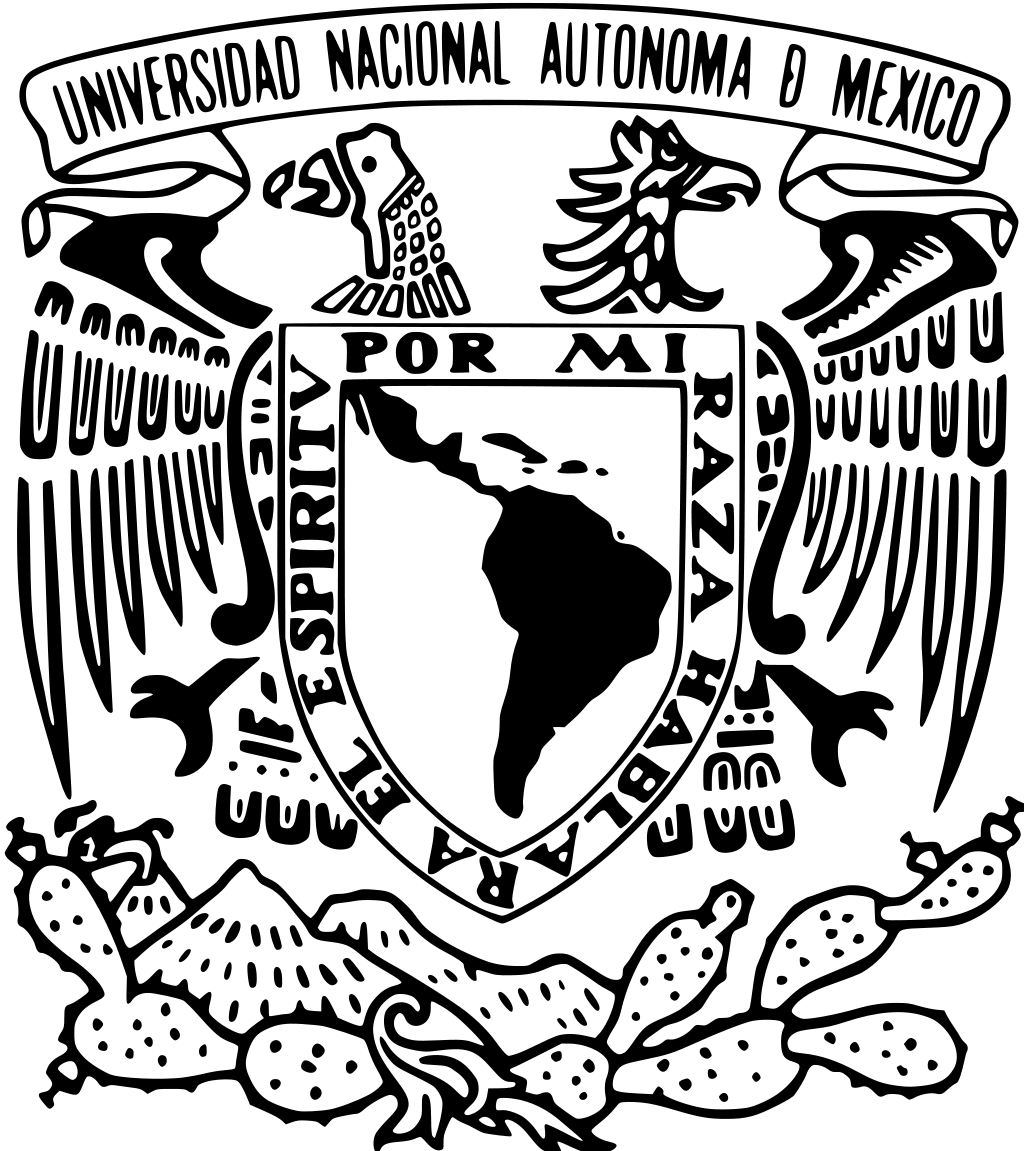
\includegraphics[width=0.50\textwidth]{unam_logo.png}\par
    \vspace{1cm}
    {\scshape\Large Universidad Nacional Autónoma de México \par}
    \vspace{1cm}
    {\scshape\Large Facultad de Ciencias \par}
    \vspace{1.5cm}
    {\huge\bfseries Arquitectura de Computadoras \par}
    {\huge\bfseries Tarea 1 \par}
    \vspace{2cm}
    {\Large\itshape David Rivera Morales\par}
    {\Large \itshape Christian Eulogio Sánchez \par}
    \vfill
  
\end{titlepage}




\section*{Desarrolla un circuito que simule el comportamiento de la tabla de verdad del Si y solo si P ⇐⇒ Q. Para este ejercicio solo puedes usar compuertas, como AND, OR, NAND, ect.}


\begin{table}[h]
\centering
\begin{tabular}{cc|c}
\hline
P & Q & \( P \Leftrightarrow Q \) \\
\hline
0 & 0 & 1 \\
0 & 1 & 0 \\
1 & 0 & 0 \\
1 & 1 & 1 \\
\hline
\end{tabular}
\caption{Tabla de verdad del bicondicional}
\label{tab:truth_table_biconditional}
\end{table}

\begin{table}[h]
\centering
\begin{tabular}{c|c|c}
\multicolumn{1}{r}{} & \multicolumn{1}{c}{Q} & \multicolumn{1}{c}{Q'} \\ \cline{2-3}
P  & 1 & 0 \\ \cline{2-3}
P' & 0 & 1 \\ \cline{2-3}
\end{tabular}
\caption{Mapa de Karnaugh del bicondicional}
\label{tab:kmap_biconditional}
\end{table}


\section*{Preguntas sobre Transistores y Circuitos}

\begin{enumerate}
    \item \textbf{¿Cuál es la diferencia entre un transistor P y uno N?} \\
    La principal diferencia entre un transistor tipo P (PMOS) y uno tipo N (NMOS) radica en el tipo de material semiconductor que utilizan y en cómo responden a las señales eléctricas. Los transistores tipo N usan silicio dopado con impurezas que les otorgan un exceso de electrones (portadores de carga negativa), mientras que los transistores tipo P usan silicio dopado de manera que les falten electrones, creando "huecos" que actúan como portadores de carga positiva. En un transistor NMOS, la corriente fluye más fácilmente cuando se aplica una tensión positiva a la puerta, mientras que en un PMOS, la corriente fluye cuando la tensión en la puerta es baja o negativa respecto al sustrato. Esto significa que los transistores tipo N son generalmente más eficientes y se usan en aplicaciones de mayor frecuencia que los transistores tipo P.

    \item \textbf{¿Cuáles son las partes de un transistor?} \\
    Un transistor, sin importar su tipo, generalmente tiene tres partes principales:
    \begin{itemize}
        \item \textit{Emisor:} La región que emite portadores de carga (electrones o huecos) hacia la base.
        \item \textit{Base:} La región central delgada que controla el flujo de portadores de carga del emisor al colector.
        \item \textit{Colector:} La región que recoge los portadores de carga emitidos por el emisor.
    \end{itemize}

    \item \textbf{¿Por qué se dice que los mapas de Karnaugh no nos dan una garantía de que siempre nos van a devolver la expresión mínima de la función?} \\
    Se dice que los mapas de Karnaugh no garantizan siempre la expresión mínima de una función porque, aunque son una herramienta poderosa para simplificar expresiones lógicas, dependen de la habilidad del usuario para visualizar y agrupar los unos o los ceros de manera efectiva. En algunas situaciones, especialmente con funciones complejas o cuando se trabaja con un número grande de variables, puede ser difícil identificar todas las agrupaciones óptimas o se pueden pasar por alto simplificaciones adicionales. Esto puede llevar a obtener una expresión simplificada, pero no necesariamente la mínima posible.

    \item \textbf{¿Cuál es el procedimiento a seguir para desarrollar un circuito que resuelve un problema que involucre lógica combinacional?}
    \begin{enumerate}
        \item Definir el problema y las especificaciones del circuito, incluyendo las entradas y salidas deseadas.
        \item Crear la tabla de verdad que describa el comportamiento lógico del circuito.
        \item Usar la tabla de verdad para derivar una expresión lógica de la función o funciones de salida.
        \item Simplificar la expresión lógica usando técnicas como álgebra booleana o mapas de Karnaugh para hacer el circuito más eficiente.
        \item Diseñar el circuito utilizando los elementos lógicos básicos (AND, OR, NOT, NAND, NOR, etc.) basándose en la expresión simplificada.
        \item Verificar y validar el diseño del circuito mediante simulación o pruebas prácticas.
    \end{enumerate}

    \item \textbf{Si una función de conmutación se evalúa a más ceros que unos ¿Es conveniente usar minterminos o maxterminos? ¿En el caso que se evalúe a más unos que ceros?} \\
    Si una función de conmutación se evalúa a más ceros que unos, es más conveniente usar maxterminos (forma canónica de productos), ya que esto llevará a una simplificación más directa al representar las condiciones en las que la función es 0.
    Si se evalúa a más unos que ceros, entonces es conveniente usar minterminos (forma canónica de sumas), porque se simplifica mejor representando directamente las condiciones en las que la función es 1.

    \item \textbf{Analizando el trabajo realizado, ¿cuáles son los inconvenientes de desarrollar los circuitos de forma física?}
    \begin{itemize}
        \item \textit{Costo y tiempo:} El diseño, prototipado y fabricación de circuitos físicos pueden ser costosos y tardados.
        \item \textit{Complejidad y errores:} A medida que la complejidad del circuito aumenta, también lo hace la probabilidad de errores, que pueden ser difíciles y costosos de diagnosticar y corregir.
        \item \textit{Modificaciones:} Hacer cambios en los circuitos físicos puede ser complicado y puede requerir la fabricación de nuevos prototipos.
        \item \textit{Espacio y recursos:} Los circuitos físicos requieren espacio y recursos materiales, lo que puede ser un problema para diseños grandes o para la realización de múltiples prototipos.
        \item \textit{Durabilidad y fiabilidad:} Los componentes físicos pueden desgastarse o fallar, afectando la durabilidad y fiabilidad del circuito.
    \end{itemize}
\end{enumerate}

\end{document}
